\section{Experimental Results}

\begin{table*}[!h]
\caption{Comparison of accuracy of our method with four baselines on eight datasets}
\centering
\resizebox{1.0\textwidth}{!}{
\begin{tabular}{lcccccccc}
\hline
\multirow{2}{*}{Models} & \multicolumn{5}{c}{Arithmetic} & \multicolumn{1}{c}{Commonsense} & \multicolumn{2}{c}{Symbolic} \\
\cmidrule(lr){2-6}
\cmidrule(lr){7-7}
\cmidrule(lr){8-9}

& MultiArith & GSM8K & AQuA  & SingleEq & SVAMP & Strategy & Letter & Coin \\
\hline
Zero-Shot & 40$\pm$1.0 & 30.4$\pm$1.7 & 29.9$\pm$1.8 & 82.7$\pm$1.3 & 56$\pm$1.0 & 59$\pm$1.0 & 43$\pm$1.0 & 79.8$\pm$1.2 \\
Zero-Shot-CoT & 91.5$\pm$1.2 & 64.1$\pm$1.1 & 55.6$\pm$1.3 & 87.43$\pm$0.25 & 79.99$\pm$1.41 & 58.34$\pm$1.56 & 69$\pm$1.0 & 93$\pm$1.0  \\
Manual-CoT & 93.5$\pm$0.1 & 64.7$\pm$1.5 & 55$\pm$1.0 & 92.1$\pm$0.2 & 82.3$\pm$0.3 & 65.3$\pm$1.4 & 75$\pm$0.0 & 92.7$\pm$0.1 \\
Auto-CoT & 94$\pm$0.0 & 65.8$\pm$0.9 & 65$\pm$0.0 & 92$\pm$0.0 & 81.9$\pm$0.3 & 65.3$\pm$0.5 & 73.5$\pm$0.2 & 93$\pm$0.0 \\
\hline
Must Think More Step (Zero-Shot-CoT)  & 95.2$\pm$0.3 & 76.1$\pm$0.1 & 62.11$\pm$0.24& 87.43$\pm$0.16 & 79.99$\pm$0.18 & 72.6$\pm$0.21 & 69$\pm$0.0 & 97$\pm$0.0 \\
Add Reasoning Step (Manual-CoT) & 97$\pm$0.0 & 70.1$\pm$0.3 & 62.5$\pm$0.5 & 88.97$\pm$0.27 & 85.2$\pm$0.2 & 68.86$\pm$0.27 & 77.8$\pm$0.4 & 97.3$\pm$0.1 \\
Add Reasoning Step (Auto-CoT) & 97.2$\pm$0.1 & 78.8$\pm$0.2 & 64.03$\pm$0.36 & 92.71$\pm$0.14 & 83.7$\pm$0.2 & 70.26$\pm$0.19 & 71.2 $\pm$0.5& 99$\pm$0.0 \\
\hline
\end{tabular}%
}
\label{tab:main-results}
\end{table*}
We conduct experiments to answer the following research questions: RO1: What is the relationship of rational reasoning steps in demonstrations with CoT performance? (Section 4.2) RO2: Can we confirm that the reasoning steps are the only factor that affects LLM performance? (Section 4.3) RO3: Will compressing reasoning steps in few-shot demonstrations hurt LLM performance? (Section 4.4), RO4: Can we observe the scaling phenomenon, i.e., the required reasoning steps be related to the size of the LLMs? (Section 4.5) and RO5: What is the influence of questions in rationale towards the LLM reasoning ability? (Section 4.6)

\begin{table*}[!h]
\caption{The Case of Wrong Prompt, change one of the step in the chain of thought and preserve overall coherence}
\resizebox{1.0\textwidth}{!}{
\label{tab:case-wrong}
\begin{tabular}{|l|l|c|c|}
\hline
\multicolumn{1}{|c|}{Original Prompt}                                & \multicolumn{1}{|c|}{Wrong Prompt}  \\ \hline
\begin{tabular}[c]{@{}l@{}}\textbf{Q:} Joan has 10 books. Tom has 38 books. \\How many books do they have?\\
\textbf{Rationale:} Let’s think step by step. Joan has 10 books.\\
Tom has 38 books. we have equation books = 10 + 38 = 48. \\
They have 10 + 38 = 48 books together.\\ \textbf{Q:} Megan had 217 markers. Robert gave her 109 more markers.\\
How many markers does Megan have altogether?\end{tabular}  & {\begin{tabular}[c]{@{}l@{}}\textbf{Q:} Joan has 10 books. Tom has 38 books. \\How many books do they have?\\
\textbf{Rationale:} Let’s think step by step. Joan has 10 books.\\
Tom has 38 books. we have equation books = 10 + \textcolor{red}{8} = 48. \\
They have 10 + 38 = 48 books together.\\
\textbf{Q:} Megan had 217 markers. Robert gave her 109 more markers.\\
How many markers does Megan have altogether?\end{tabular}}  \\ \hline
\end{tabular}}
\end{table*}
\begin{figure*}[!h]

	%
	\subfigbottomskip=2pt %

	\subfigcapskip=-2pt %
	\subfigure[MultiArith]{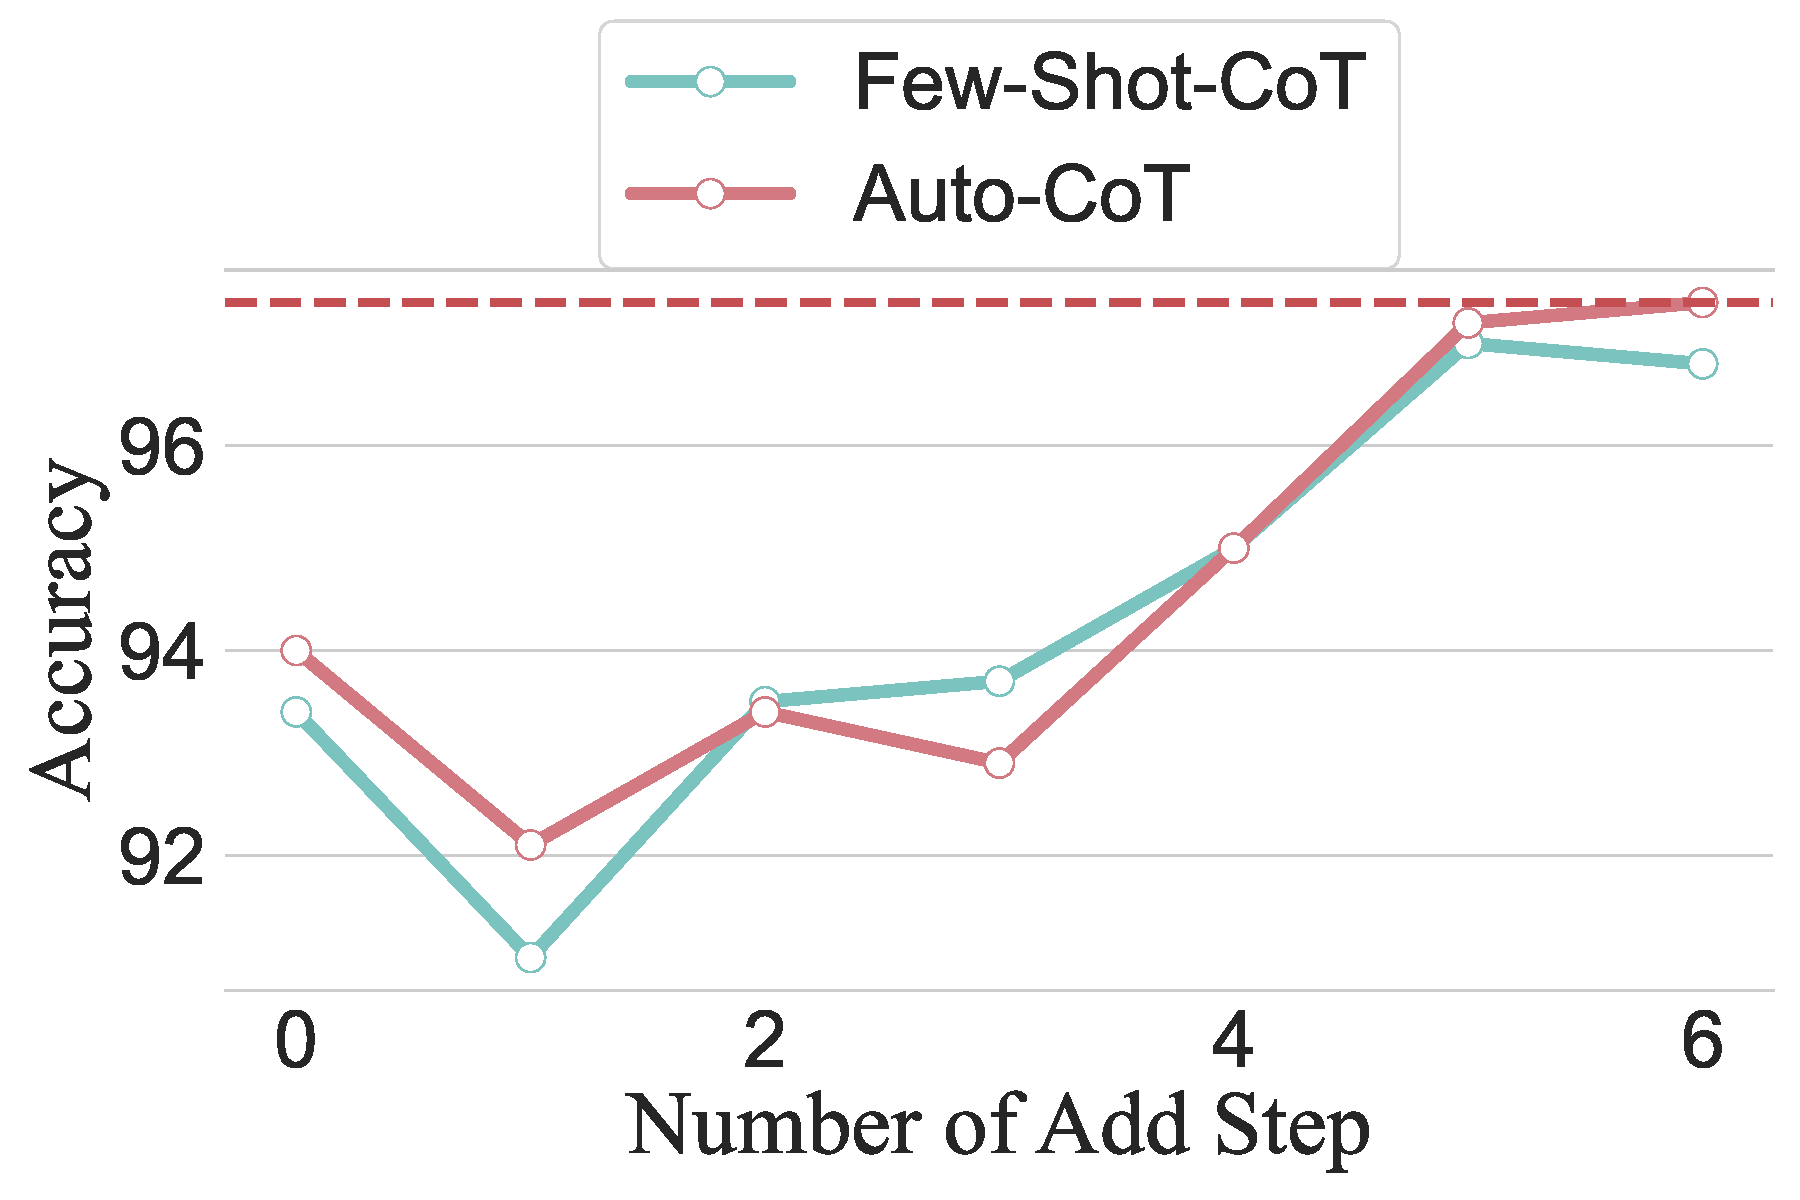
\includegraphics[width=0.24\linewidth]{MultiArith.pdf}}
	\subfigure[GSM8K]{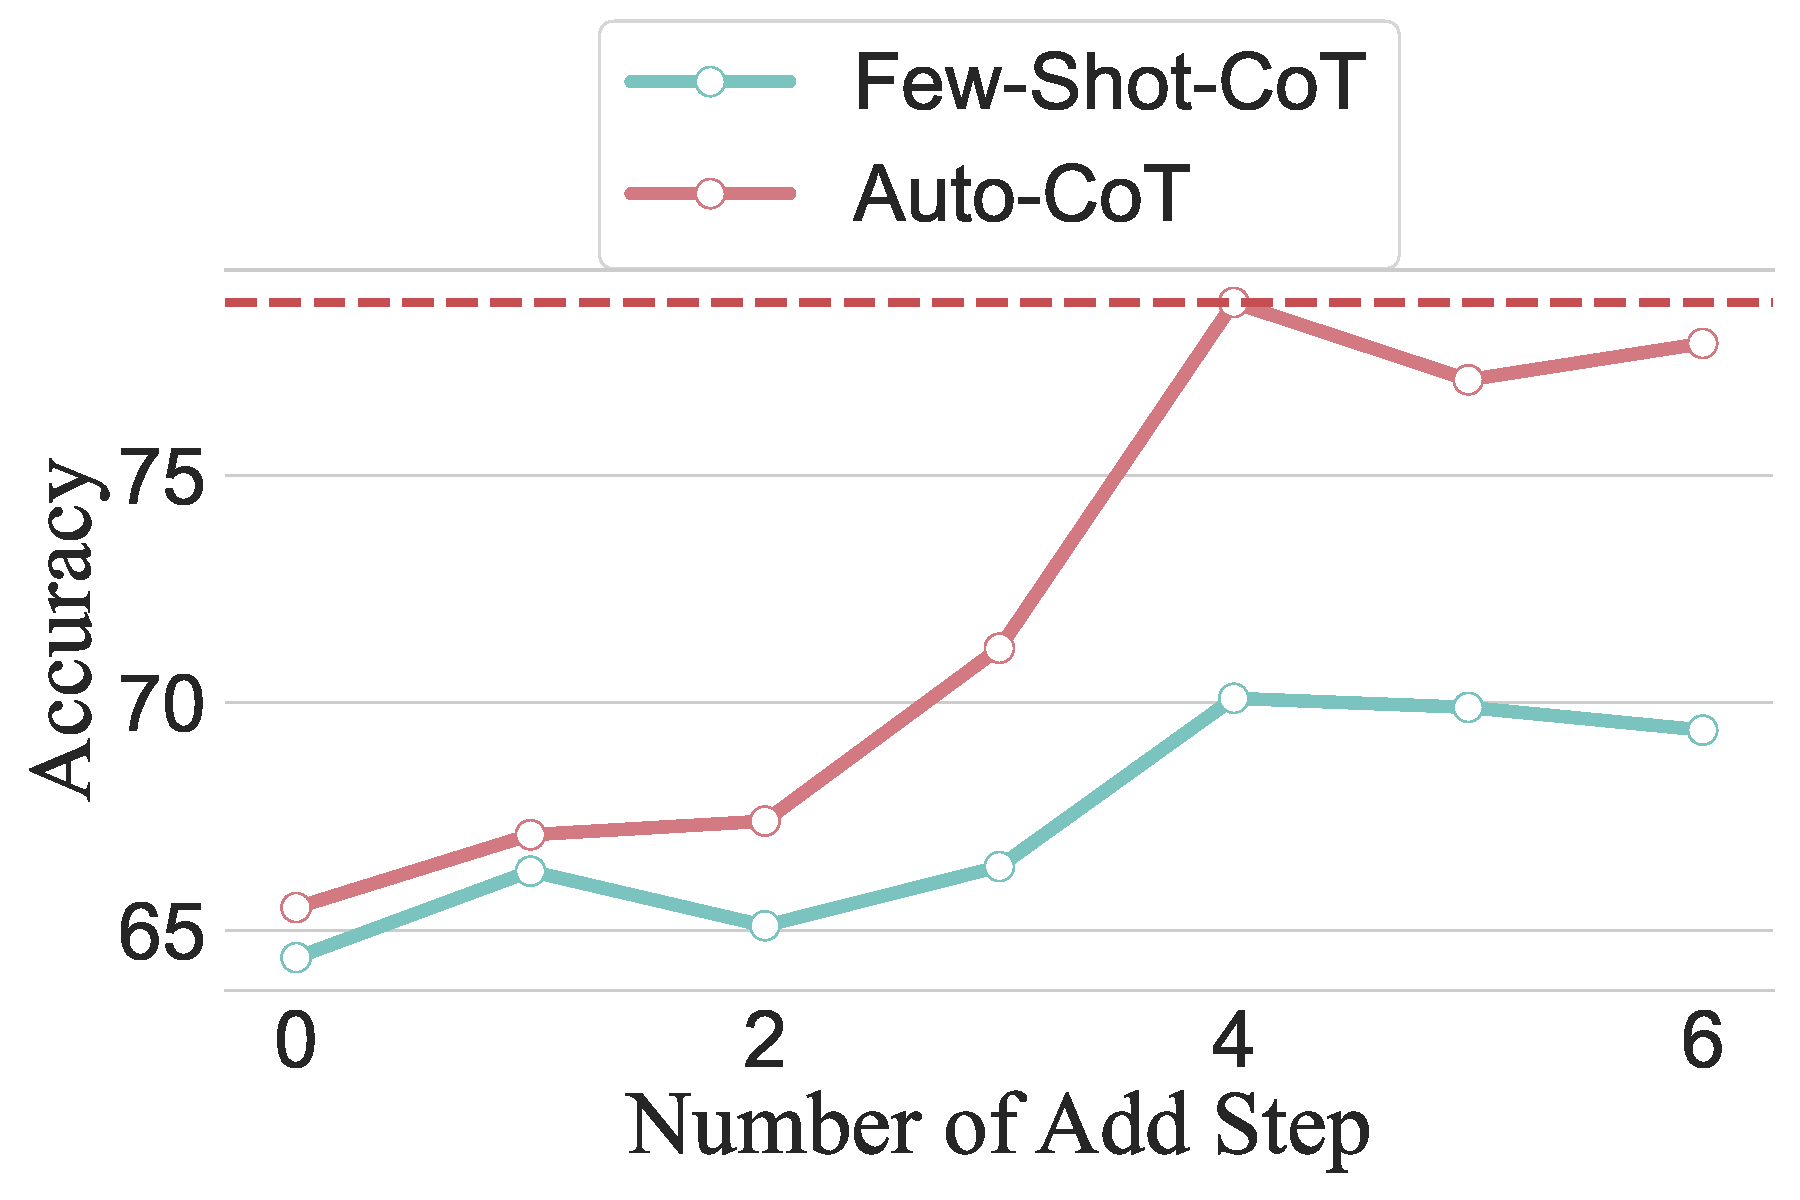
\includegraphics[width=0.24\linewidth]{GSM8K.pdf}}
	  \subfigure[AQuA]{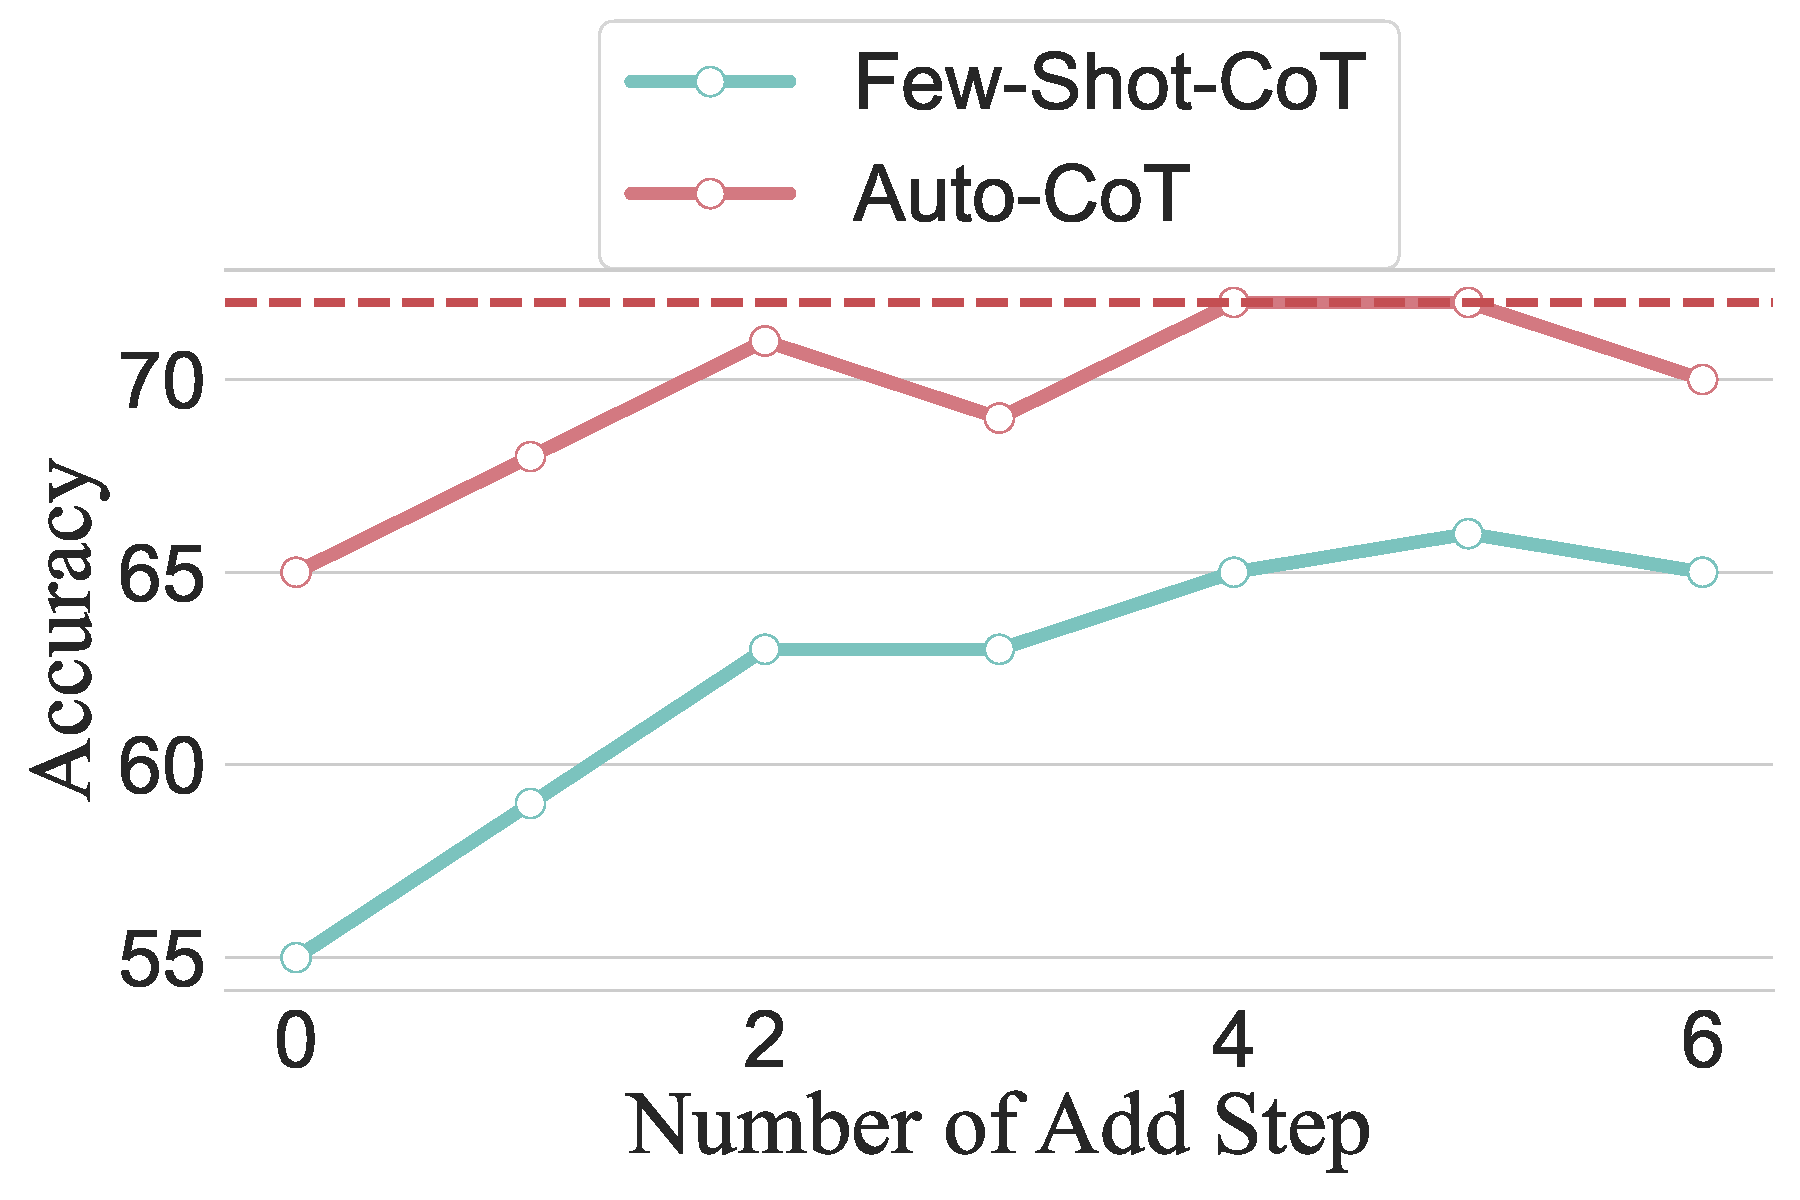
\includegraphics[width=0.24\linewidth]{AQuA.pdf}}
        \subfigure[SingleEq]{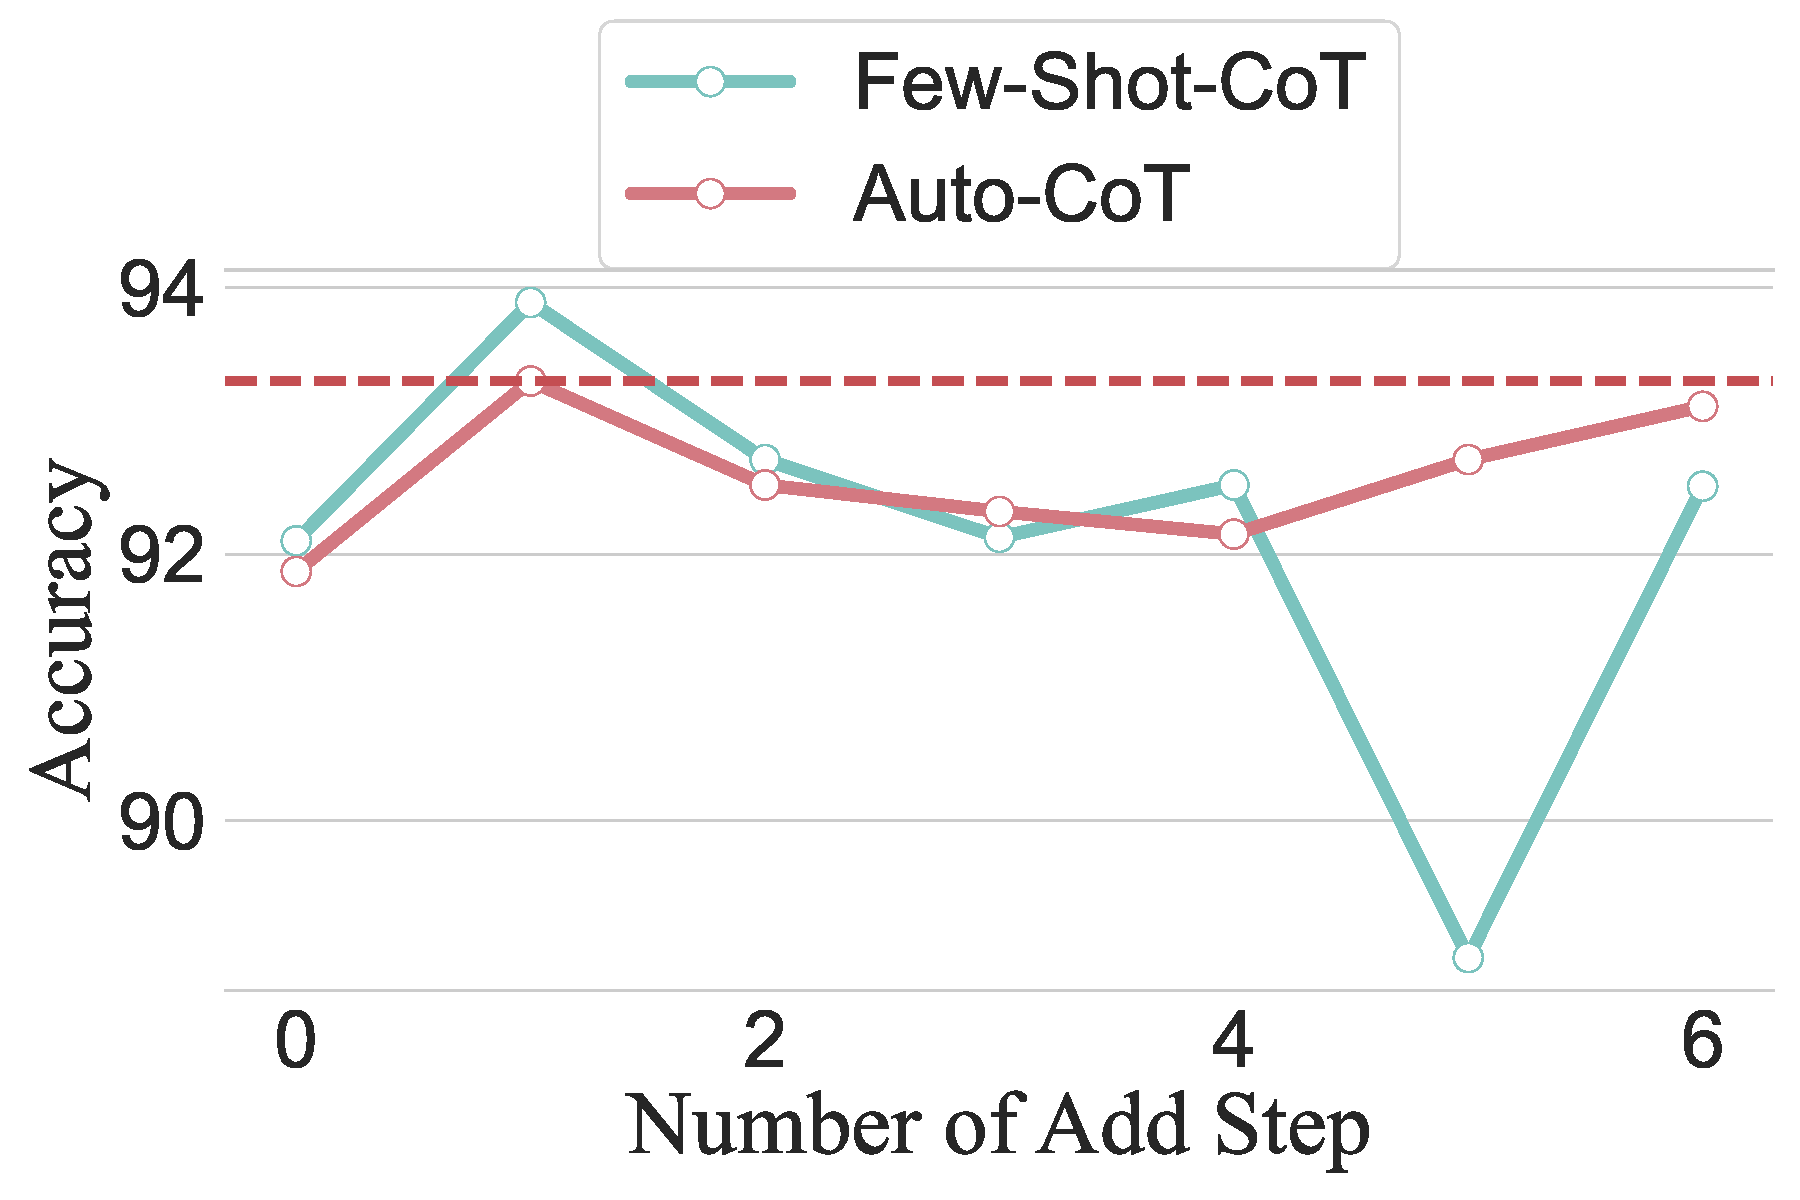
\includegraphics[width=0.24\linewidth]{SingleEq.pdf}}

	\subfigure[SAVMP]{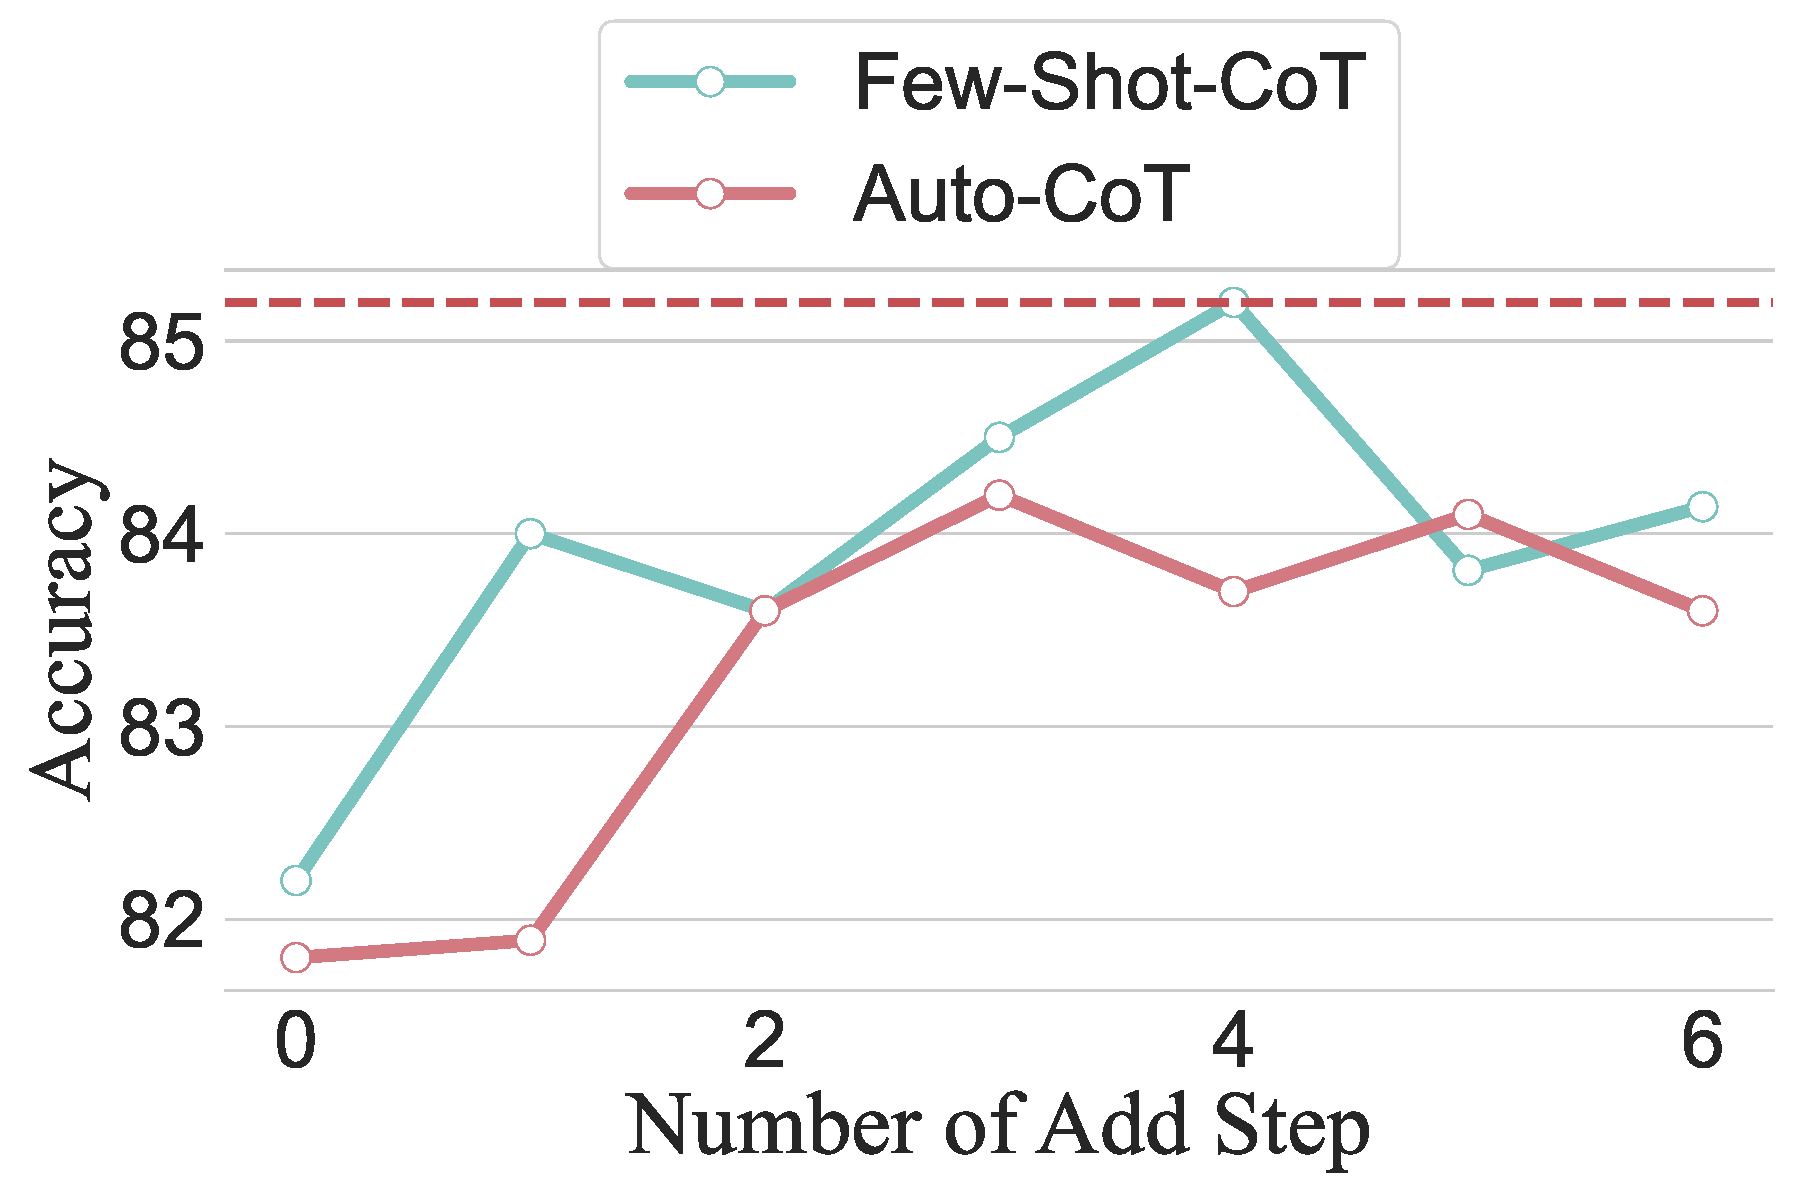
\includegraphics[width=0.24\linewidth]{svamp.pdf}}
	\subfigure[strategyqa]{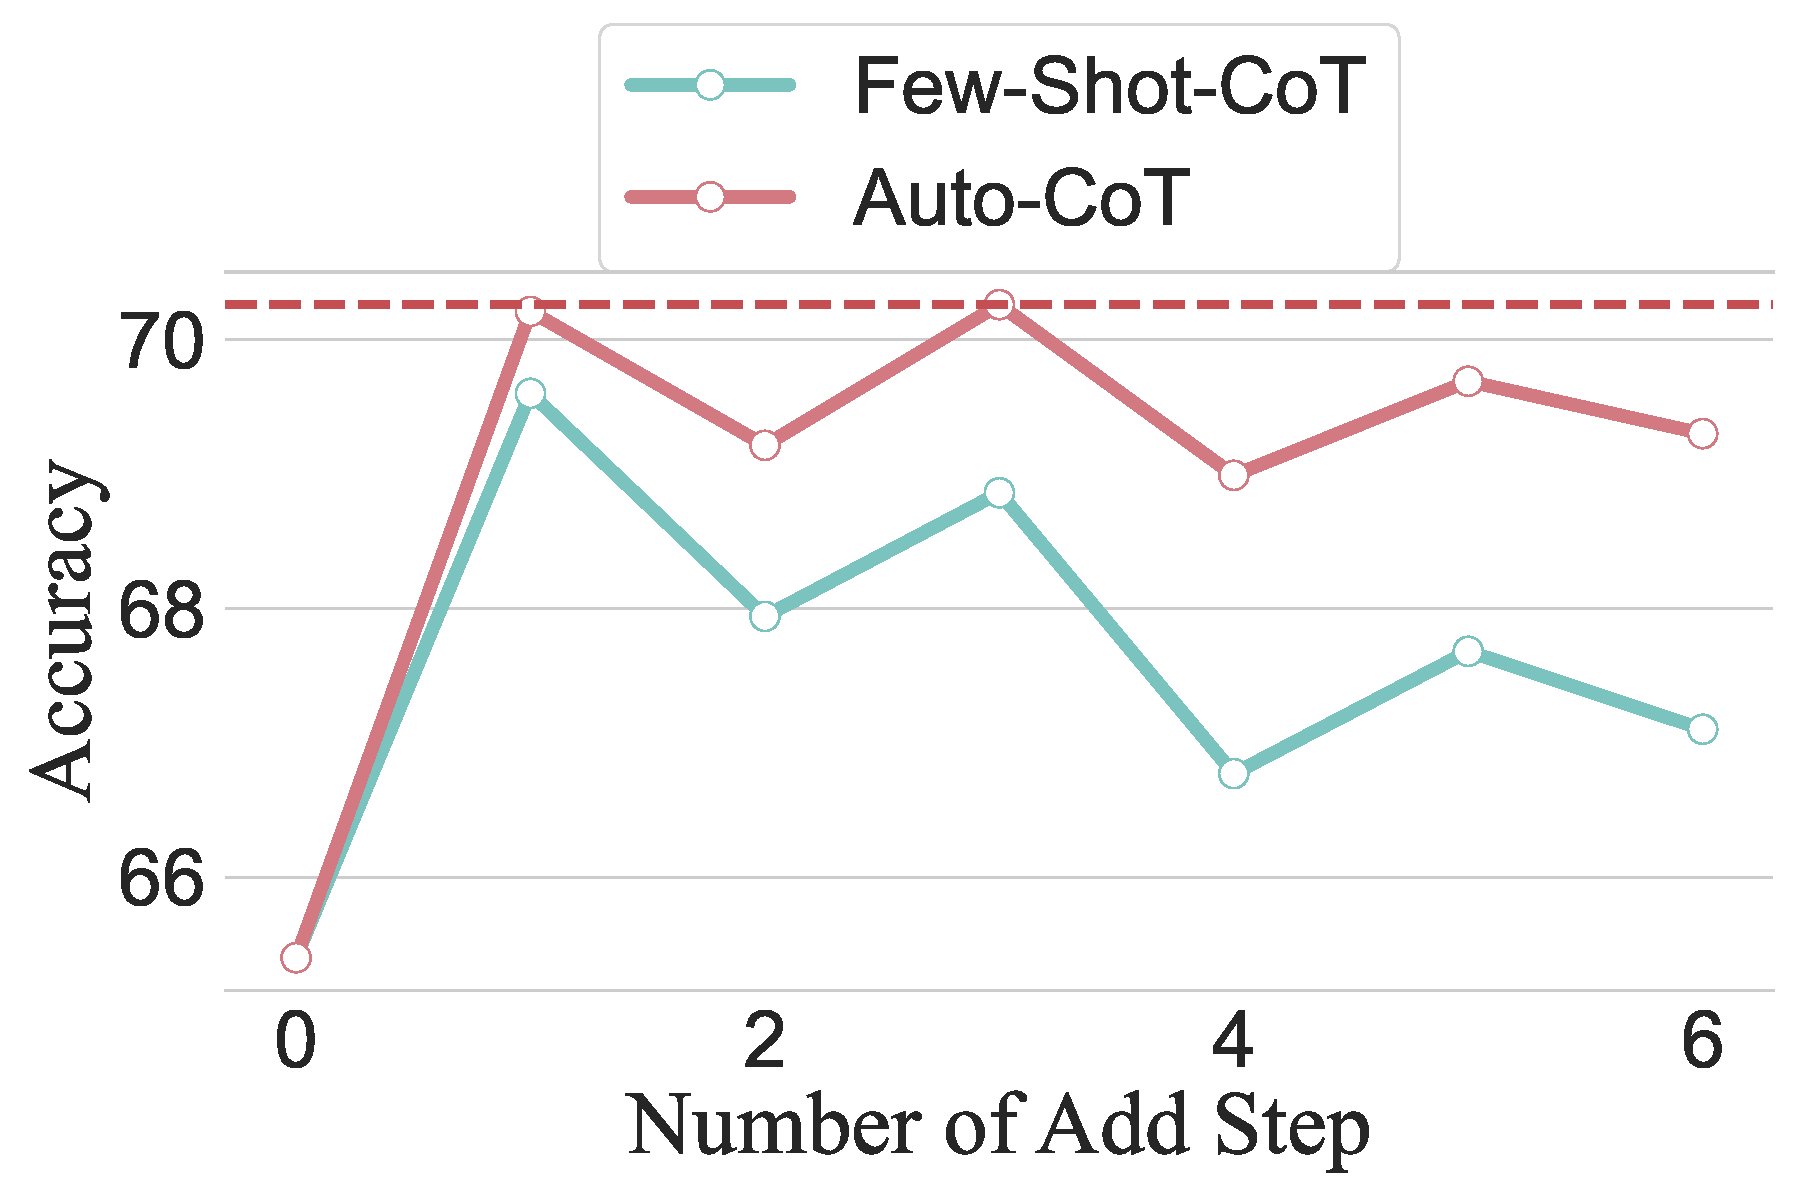
\includegraphics[width=0.24\linewidth]{strategyqa.pdf}}
	\subfigure[Letter]{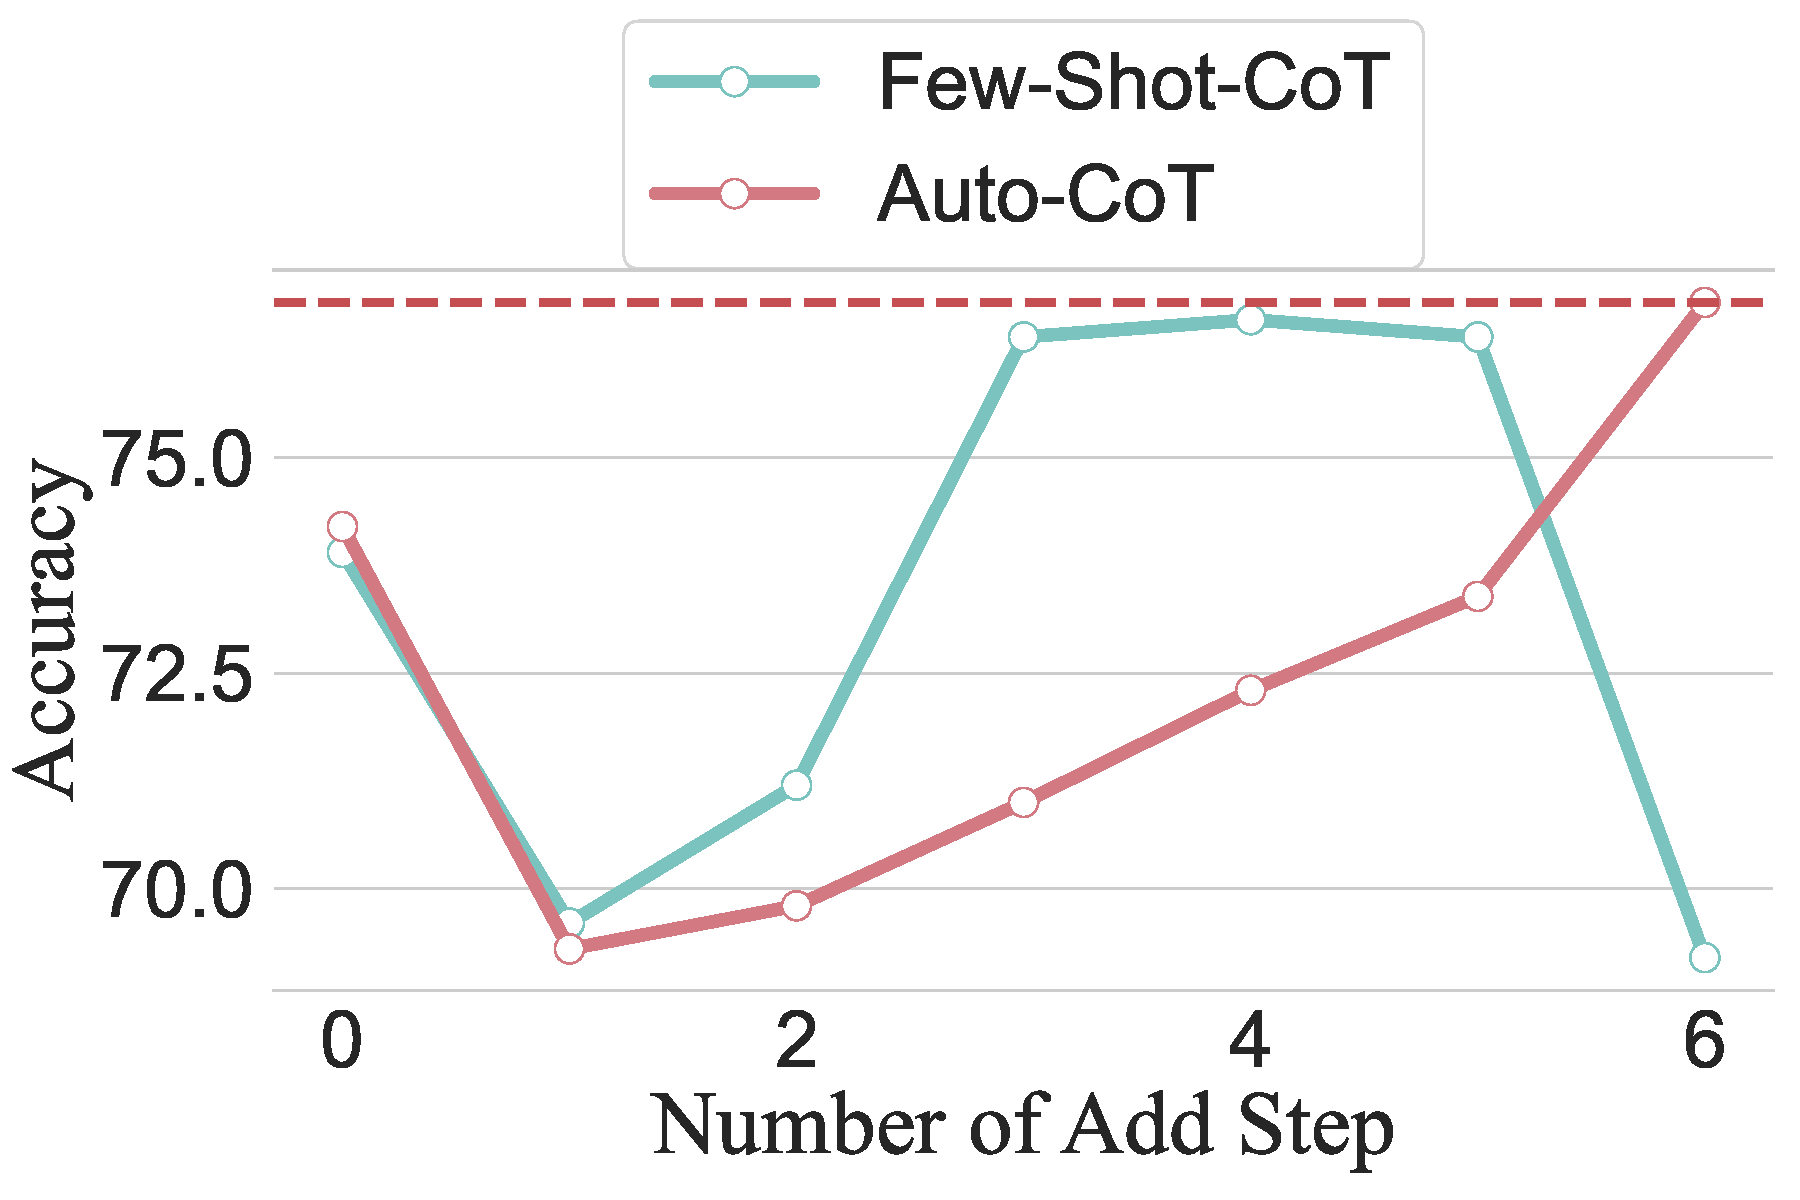
\includegraphics[width=0.24\linewidth]{last_letter.pdf}}
	\subfigure[Coin]{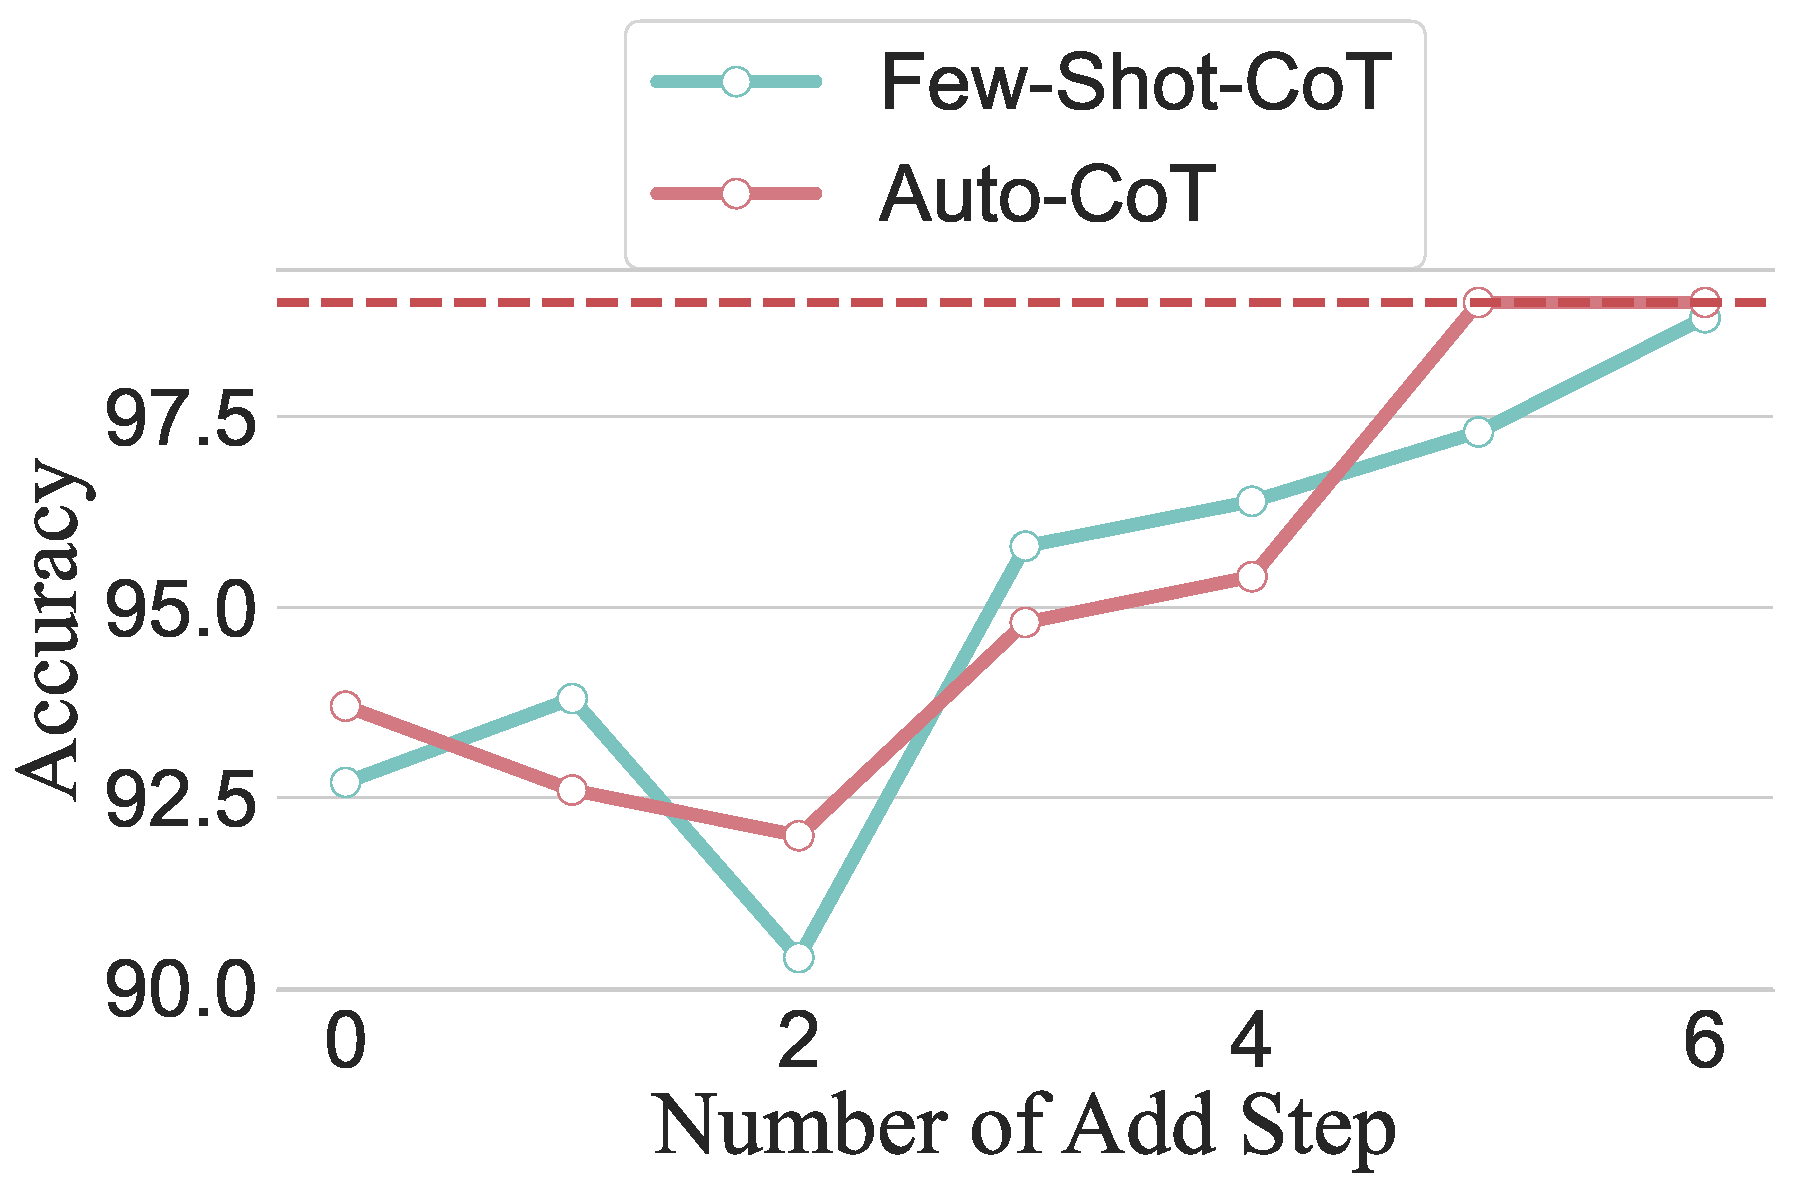
\includegraphics[width=0.24\linewidth]{coin_flip.pdf}}
\caption{Linear Relationship Between Step Quantity and Accuracy}
\label{figure1}
\end{figure*}

\subsection{Experimental Setups}
\label{section4.1}
We introduce the general experimental setups.

\noindent
\textbf{Datasets and Models}.\, We evaluate our proposal on eight dataset (MultiArith \cite{roy2015solving}, GSM8K \cite{cobbe2021training}, AQuA \cite{ling2017program}, SingleEq \cite{koncel2015parsing}, SAVMP \cite{patel2021nlp}, Letter \cite{wei2022chain}, Coin \cite{wei2022chain}, Strategyqa \cite{geva2021did}). We employ three models to validate the performance of our proposed method, which are: text-davinci-002~\cite{brown2020language}, GPT-3.5-turbo-1106 \cite{ouyang2022training}, GPT-4 \cite{openai2023gpt}.  All models are accessed via the OpenAI API key.

\vspace{2pt}
\noindent
\textbf{Prompt}.\, We have shown the proposed process pipeline in Section~3 Analyzing Methods. The experimental part follows the same approach.

\vspace{2pt}
\noindent
\textbf{Baselines}.\, We compare our methods with four baseline methods: Zero-Shot \cite{kojima2023large}, Zero-Shot-CoT \cite{kojima2023large}, Manual-CoT \cite{wei2022chain}, Auto-CoT \cite{zhang2022automatic}. The results are in the ~\autoref{tab:main-results}.

\vspace{2pt}
\noindent
\textbf{Evaluation Metrics}.\,
Accuracy is used to assess a model's ability on classification tasks and is commonly used for multichoice and yes/no tests:
$
\text{Accuracy} = {N_{\text{correct}}}/{N_{\text{total}}}.
$

\vspace{2pt}
\noindent
\textbf{Implementation Details}:

\begin{itemize}[leftmargin=*]\setlength\itemsep{-0.3em}
\item Add reasoning steps: This process deploys GPT-4 to modify the Zero-Shot-CoT prompt demo generated by ``let's think step by step" to contain the five reasoning steps we mentioned in Section~\ref{sec:methods} so that we can define the number of steps and the types of steps to be contained in the demo. We then input the demo as a prompt. We completed the following experiment with this approach.

\item Reasoning-Step Compression: In the expressing experiment, we focused on executing a compression attack on the rationale inference chain within the few-shot CoT. The process involved randomly selecting two consecutive sentences and employing GPT-4 to effectively merge them. We then input the prompt: ``Please compress the following two sentences without losing any information, and make them as concise as possible''. This method was designed to implement a targeted compression on the reasoning chain.

\item
Answer cleaning: We follow the structure proposed by Zero-Shot-CoT to select the final answer. After the model response output is obtained, this structure selects only part of the answer that first satisfies the answer format.

\end{itemize}

\subsection{Relationship Between Steps and Accuracy}
\label{section4.2}
\autoref{tab:main-results} compares accuracy on eight datasets from three categories of reasoning tasks using GPT-3.5-turbo-1106. All results are averaged over three random runs. Our SOTA results are based on experimental results from the optimal performance step for each data set. Our zero-shot CoT is based on Section 2.1, and the Add Reasoning Step (Manual-CoT), and Add Reasoning Step (Auto-CoT) is based on Section 2.2.\\

Benefiting from the fact that we have standardized the thought chain process, it is possible to quantify the increase in accuracy due to the increased steps in rationales of COT demonstrations. We conducted experiments to answer the RO1: What is the relationship of rational reason-ing steps in demonstrations with CoT performance? This experiment is completed with GPT-3.5-turbo-1106, and the results are given in ~\autoref{figure1}. We found that LLM reasoning ability improves in all datasets during an effective CoT process, i.e. with the addition of up to six steps of additional thought processes. In other words, we found a certain linear relationship between accuracy and CoT complexity.

\subsection{Effect of Prompt with Wrong Answer}
\label{section4.3}
%
To answer RO2: Are reasoning steps the only factor that affects LLM performance? We made the following attempt. Change a step in the prompt to an incorrect answer to see if it affects the chain of thought. So, for this experiment, we change all the prompts to carry one error. For a concrete example, check the ~\autoref{tab:case-wrong}. For Arithmetic-type questions, even if there is a deviation in one of the results of the prompt, the effect on the chain of thought in the reasoning process is minimal, so we believe that the large language model learns more about the chain of thought patterns in the prompt than the single computation when solving Arithmetic-type problems. For logic problems similar to those in the Coin dataset, a deviation in one of the prompt's results often brings about the fragmentation of the entire chain of thought. We completed this experiment with GPT-3.5-turbo-1106 and guaranteed performance based on the optimal number of steps for each data set derived from the previous experiment. The results are shown in ~\autoref{fig:wrong-prompt}.
%
\begin{figure}[t]
    \centering
    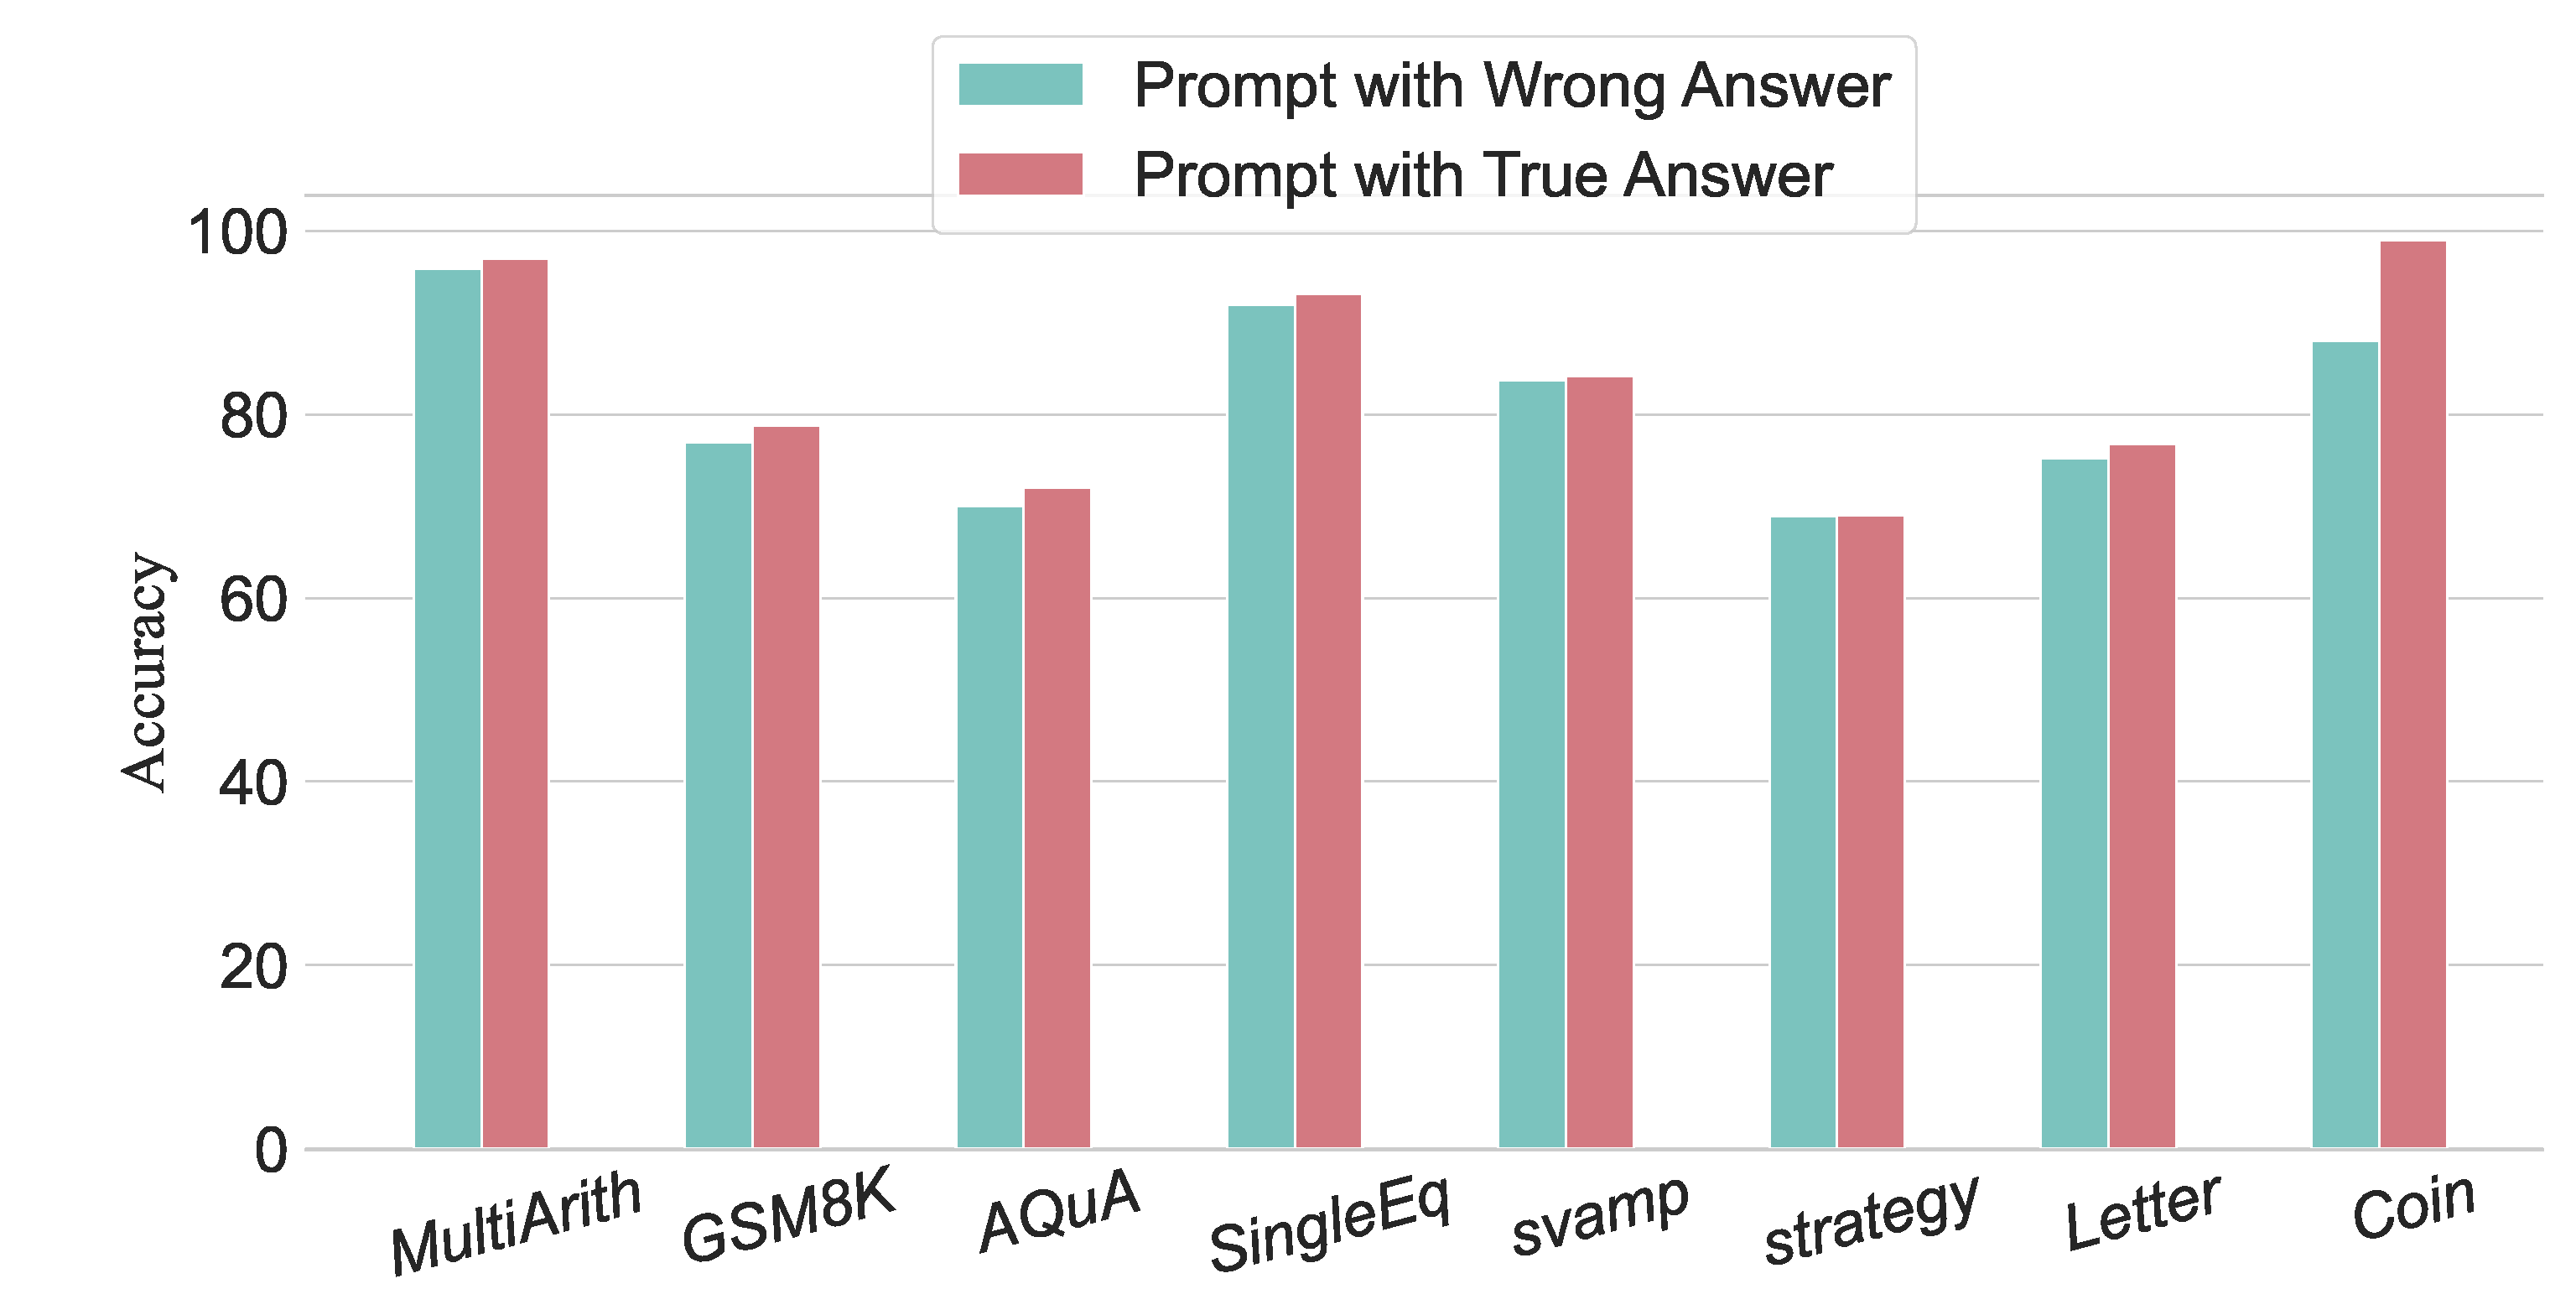
\includegraphics[width=1\linewidth]{wrong_answer.pdf}
\caption{Compare the accuracy of the prompt with the true answer and the prompt with the wrong answer}
\label{fig:wrong-prompt}
\end{figure}

\subsection{Compressing Reasoning Steps }
\label{section4.4}
\begin{table*}[!h]
\small
\caption{Making deliberate alterations to sample questions}
\resizebox{\textwidth}{!}{
\label{tab:case-wrong question}
\begin{tabular}{|m{\textwidth}|}
\hline
\textbf{Original Prompt} \\ \hline
\textbf{Q:} Wendy uploaded 45 pictures to Facebook. She put 27 pics into one album and put the rest into 9 different albums. How many pictures were in each album? \\
\textbf{Rationale:} ``Let's think step by step. First, Wendy uploaded 45 pictures in total. Second, Wendy put 27 pictures into one album. That means that Wendy put the remaining 18 pictures into 9 different albums. Each album would have 2 pictures." \\
\textbf{Pred\_ans:} ``2" \\
\textbf{Gold\_ans:} ``2" \\ \hline
\textbf{Making deliberate alterations} \\ \hline
\textbf{Q:} \textcolor{red}{Wendy uploaded 66 pictures to Facebook. She put 89 pics into one album and put the rest into 7 different albums. How many pictures were in each album?} \\
\textbf{Rationale:} ``Let's think step by step. First, Wendy uploaded 54 pictures in total. Second, Wendy put 27 pictures into one album. That means that Wendy put the remaining 12 pictures into 6 different albums. Each album would have 7 pictures." \\
\textbf{Pred\_ans:} ``2" \\
\textbf{Gold\_ans:} ``2" \\ \hline
\end{tabular}}
\end{table*}
In previous sections, we have demonstrated that increasing reasoning steps could improve the LLM reasoning accuracy. In this section, our aim is to answer RO3: Will compressing reasoning steps in few-shot demonstrations hurt LLM performance?
To this end, we conduct the reasoning steps compression experiment, and we employed the technique outlined in the experimental setup to condense the reasoning process in examples from both the baseline automated chain of thought (Auto-CoT) and the few-shot chain of thought (Few-Shot-CoT), aiming to reduce their number of inference steps. The result is shown in ~\autoref{fig:Compression}. It revealed a notable decline in performance, which regressed to a level essentially equivalent to that achieved by the zero-shot method. It further indicates that \emph{increasing COT rationale reasoning steps could improve COT performance and the vice versa.}
\begin{figure}[t]
    \centering
    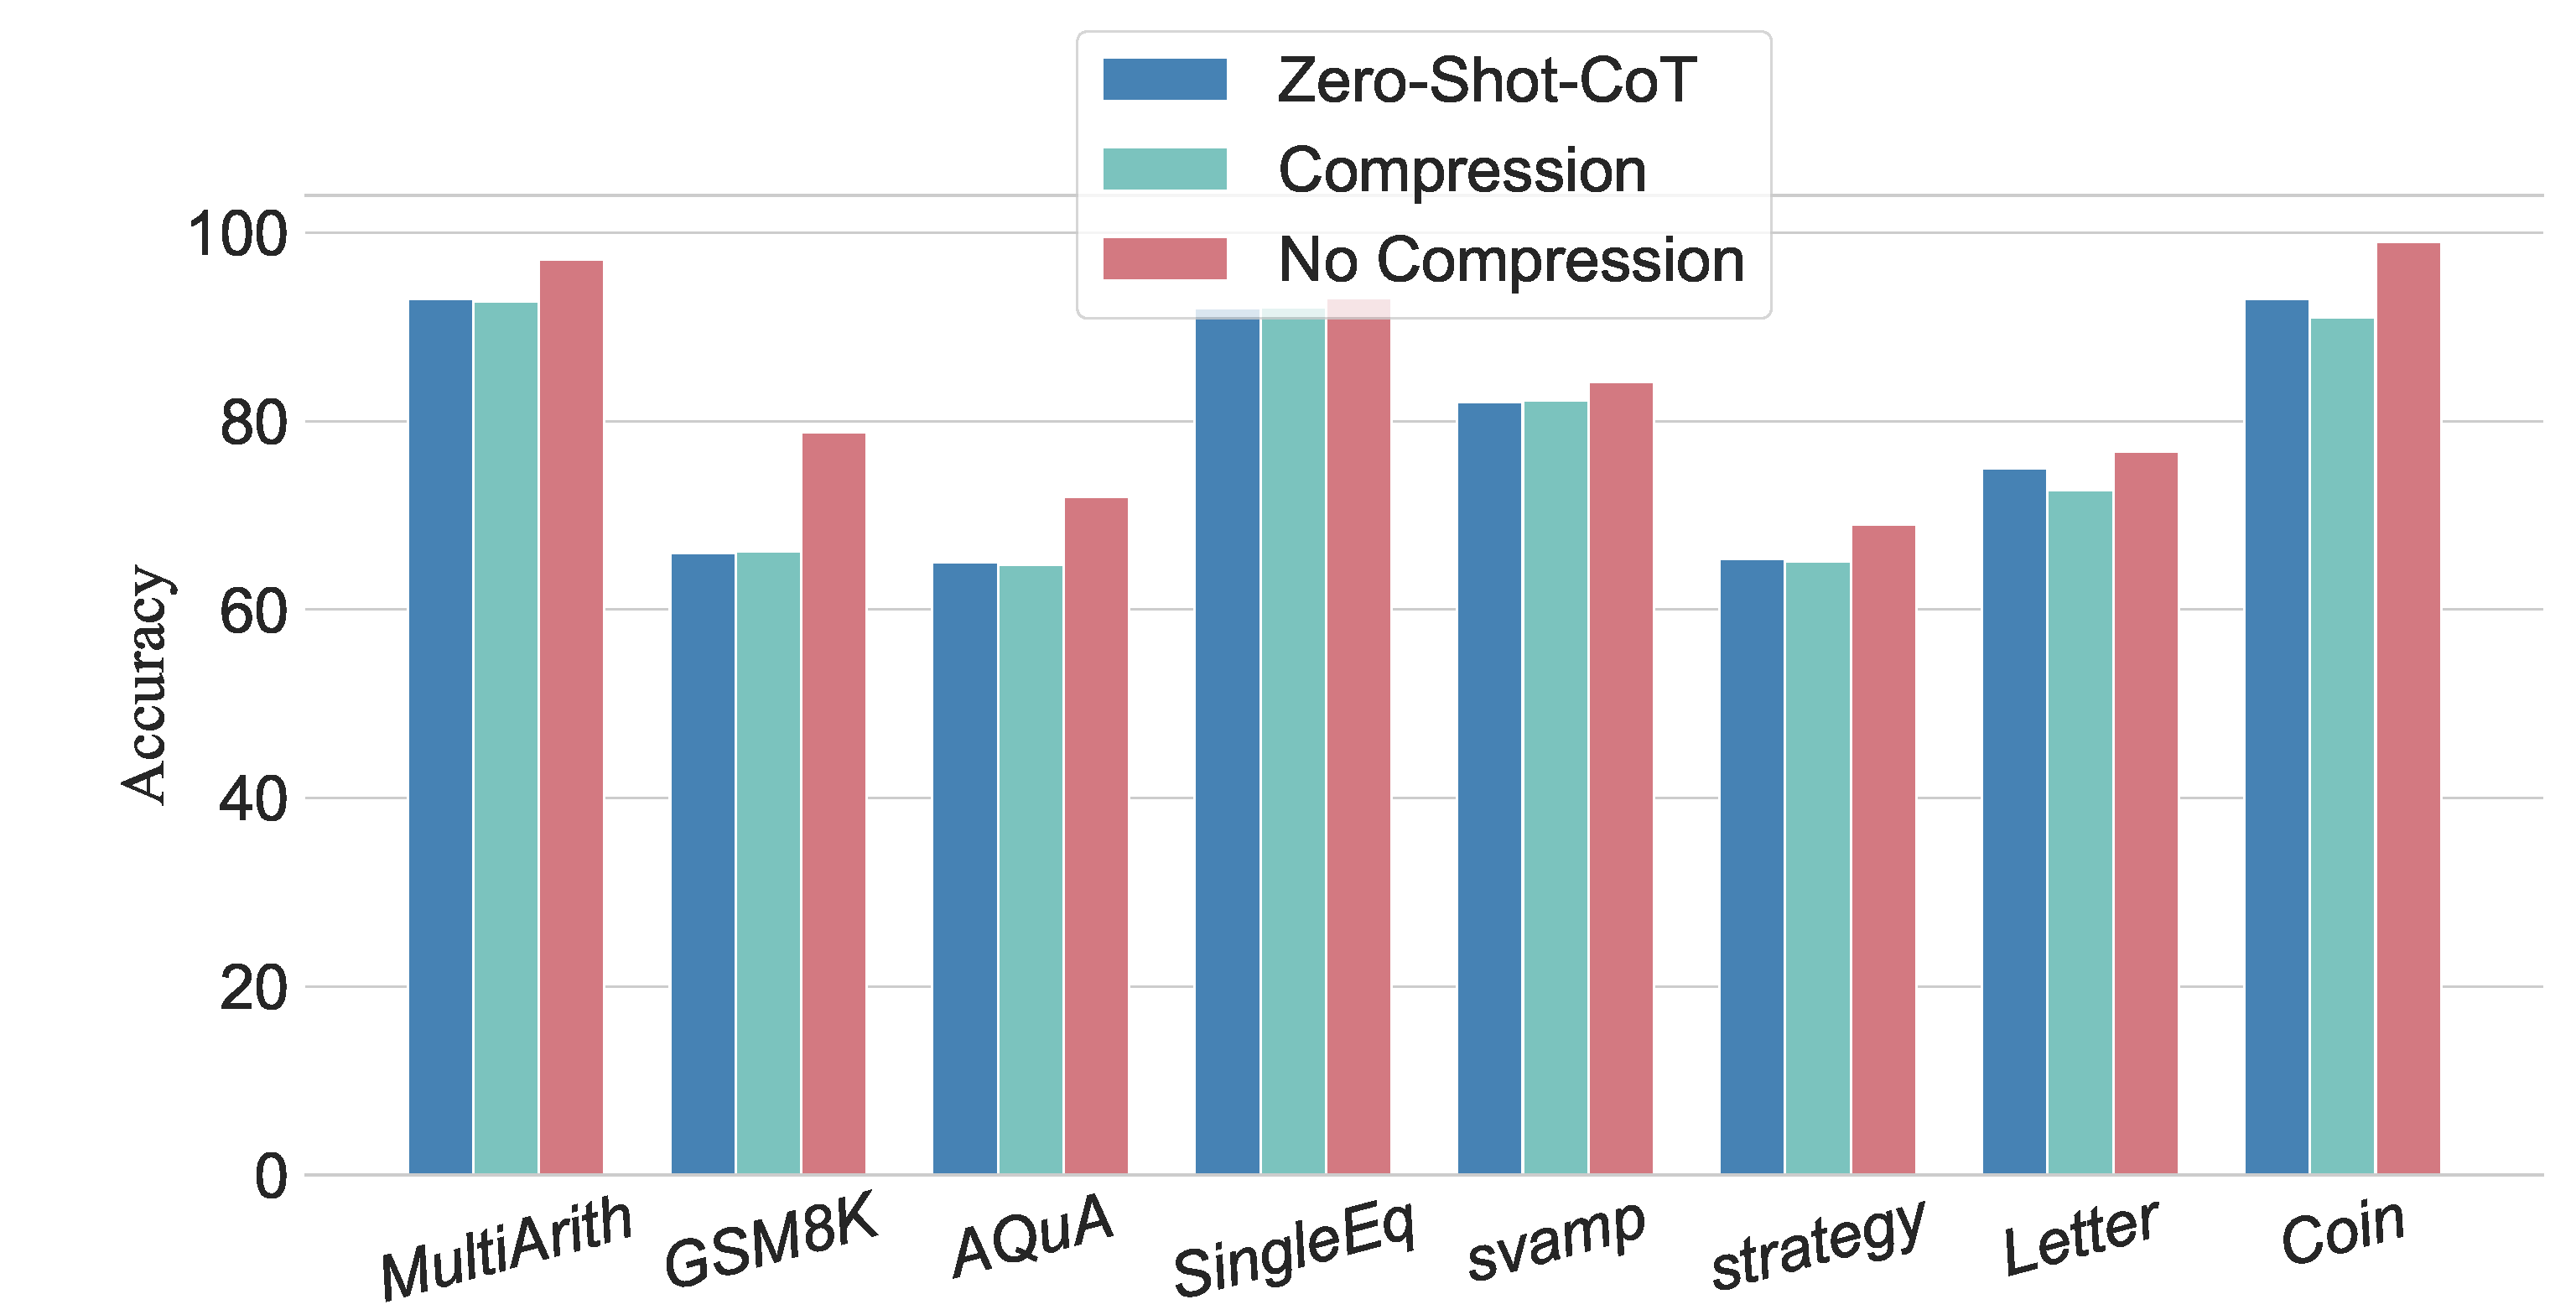
\includegraphics[width=1\linewidth]{Compression.pdf}
   \caption{Compare the accuracy of the prompt with Compression and the prompt with No Compression}
    \label{fig:Compression}
\end{figure}

\subsection{Performance on Different Size Models}
%
\label{section4.5}

In this chapter, our focus is to answer RO4: Can we observe the scaling phenomenon, i.e., the required reasoning steps be related to the size of the LLMs? We examine the average number of inference steps utilized in various models, including text-davinci-002, GPT-3.5-turbo-1106, and GPT-4. We conducted experiments on GSM8K calculating the average inference step for each model to reach peak performance. This dataset has the largest performance difference with text-davinci-002, GPT-3.5-turbo-1106, and GPT-4 out of our 8 datasets. It can be observed that the model with the worst initial performance, text-davinci-002, our strategy has the highest boosting effect. For the model with the best initial performance, GPT-4, has the highest tolerance to our strategy (no performance decreases). We show the result in ~\autoref{diff_model}.

\begin{figure}[t]
    \centering
    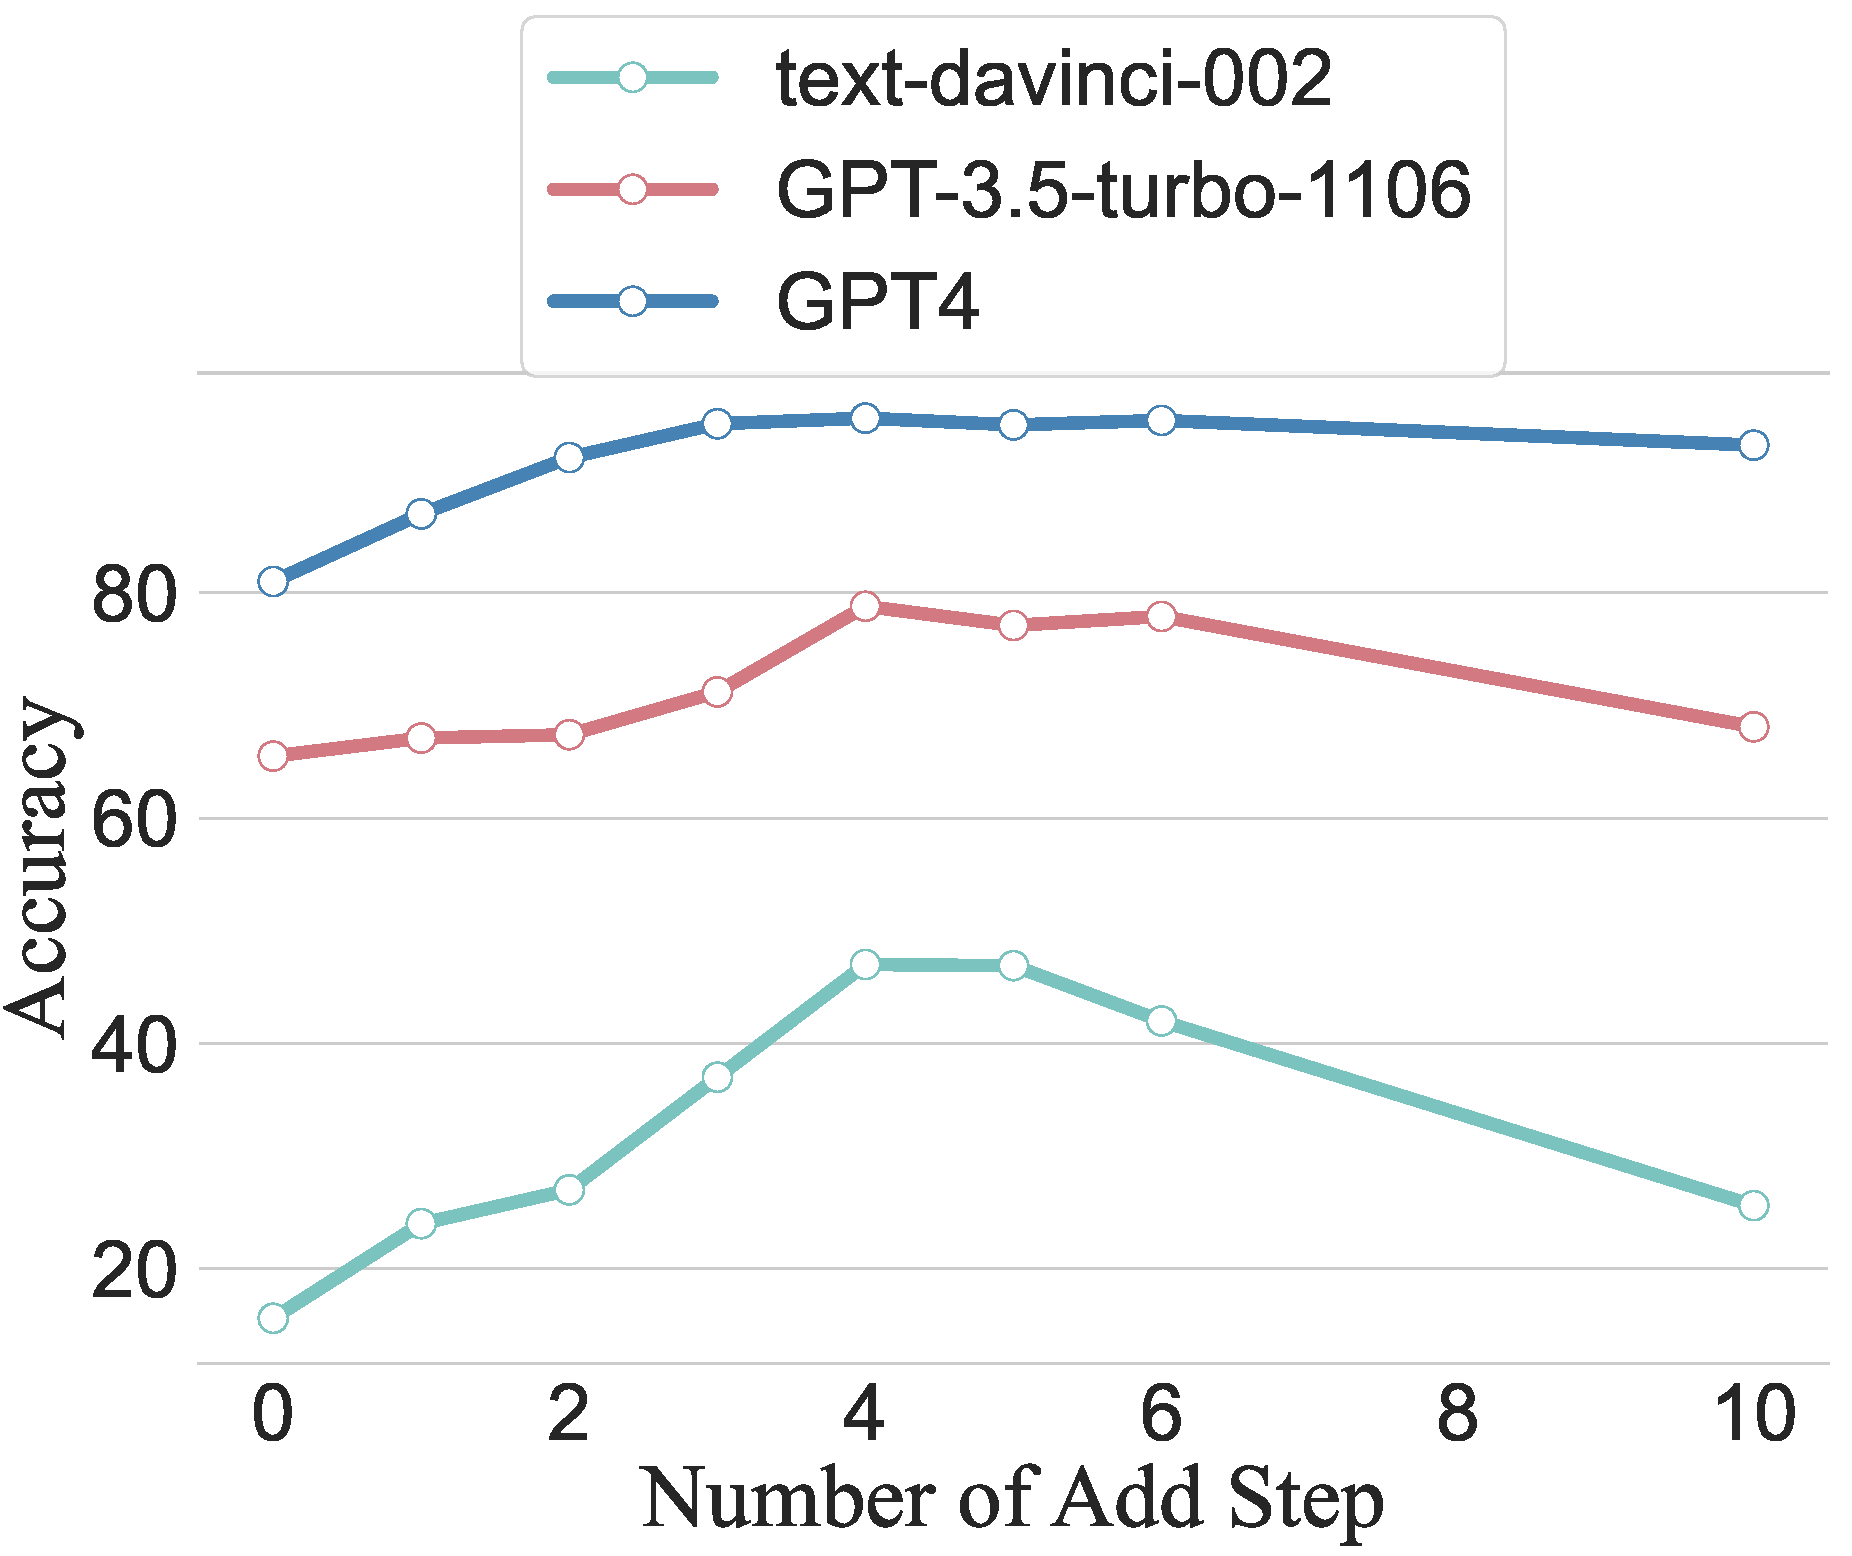
\includegraphics[width=0.75\linewidth]{DIFF_MODEL.pdf}
    \caption{Comparing the accuracy with different size model on dataset GSM8K.}
    \label{diff_model}
\end{figure}

\subsection{Influence of Questions in CoT Examples}
\label{section4.6}

In our case study, we aim to answer RO5: What is the influence of questions in rationale towards the LLM reasoning ability? We want to explore whether changing the reasoning in CoT will affect CoT performance. Since we are mainly studying the impact of the inference step on performance, we need to confirm that the question has no impact on performance. So we have chosen two datasets and two CoT methods (auto-CoT and few-shot-CoT) for this investigation: MultiArith \cite{roy2015solving} and GSM8K \cite{cobbe2021training} in GPT-3.5-turbo-1106. Our experimental approach involves making deliberate alterations to sample questions within these mathematical datasets, such as varying the content of the questions in ~\autoref{tab:case-wrong question}. Remarkably, initial observations indicate that these modifications have only minimally impacted performance like ~\autoref{tab:case1}.

This preliminary finding suggests that the length of the steps involved in the reasoning process, rather than the nature of the questions themselves, predominantly influences the reasoning capabilities of large-scale models.

\begin{table}[t]
\small
\centering
\caption{Accuracy comparison of models on different datasets}
\begin{tabular}{lcc}
\toprule
Models & MultiArith & GSM8K \\
\midrule
Zero-Shot & 40$\pm$1.0 & 30.4$\pm$1.7 \\
Zero-Shot-CoT & 91.5$\pm$1.2 & 64.1$\pm$1.1 \\
Manual-CoT & 93.5$\pm$0.1 & 64.7$\pm$1.5 \\
Auto-CoT & 94$\pm$0.0 & 65.8$\pm$0.9 \\
\hline %
Changing Question \\(Manual-CoT) & 92.9$\pm$0.1 & 62.1$\pm$1.7 \\
Changing Question \\(Auto-CoT) & 92.5$\pm$0.1 & 63.5$\pm$1.0 \\
\hline
Add Reasoning Step \\(Manual-CoT) & 97$\pm$0.0 & 70.1$\pm$0.3 \\
Add Reasoning Step \\(Auto-CoT) & 97.2$\pm$0.1 & 78.8$\pm$0.2 \\
\hline
Add Reasoning Step \\and Changing Question\\(Manual-CoT) & 96.6$\pm$0.1 & 69.6$\pm$0.2 \\
Add Reasoning Step \\and Changing Question\\(Auto-CoT) & 95.7$\pm$0.1 & 75.2$\pm$0.2 \\
\bottomrule
\end{tabular}
\label{tab:case1}
\end{table}